\subsection{Space Vector Pulse Width Modulation}

Space Vector PWM has several advantages over Sine PWM

\begin{itemize}
    \item Higher voltage utilization: SVPWM can utilize up to 15\% more DC bus voltage compared to SPWM. This means for the same DC supply voltage, an inverter with SVPWM can provide a higher output voltage.

    \item Better harmonic performance: SVPWM results in lower total harmonic distortion (THD) compared to SPWM. This leads to a better quality of the output voltage and current waveforms, which is particularly important in applications like drives where harmonics can cause heating and torque pulsations.

    \item Reduced switching losses: SVPWM requires fewer switching operations for the inverter switches compared to SPWM. This results in lower switching losses, leading to higher efficiency and reduced heating of the inverter switches.

    \item Improved dynamic response: The space vector representation used in SVPWM allows for a more precise control of the output voltage vector, leading to an improved dynamic response. This is particularly beneficial in applications like motor drives where a fast dynamic response is required.

    \item Vector control capability: SVPWM allows for vector control of the output voltage, which is not possible with SPWM. This enables more complex control strategies, such as field-oriented control (FOC), which can provide better performance in applications like motor drives.

    \item Flexibility: SVPWM allows for flexible control of the output voltage magnitude and frequency, as well as the phase relationship between the output voltage and current. This flexibility makes it suitable for a wide range of applications. 
\end{itemize}

\subsubsection{Generation of Space Vector PWM with C2000 microcontroller}

To generate space vector PWM wave for the switches C2000 series microcontroller offers a hardware level module called ePWM or enhanced PWM module. It enables to generate PWM waves with high flexibility.

To generate symmetrical waveform, the ePWM's internal timer is configured in up-down count mode.

\begin{equation}
    T_{PWM} = (2 \times TBPRD \times T_{TBCLK})
\end{equation}

\begin{equation}
    F_{PWM} = {1 \over T_{PWM}}
\end{equation}



$F_{PWM}$ - Frequency of PWM


$T_{PWM}$ - Time period of PWM


$T_{TBCLK}$ - Time base clock


$TBPRD$ - ePWM Time period


$$TBCLK = {EPWMCLK \over HSPCLKDIV \times CLKDIV}$$


$EPWMCLK$ - ePWM clock derived from system clock. System clock is $200 \, Mhz$


$HSPCLKDIV$ - High speed clock divider


$CLKDIV$ - Clock prescaler



% ePWM block in simulink
\begin{figure}[H]
    \centering
    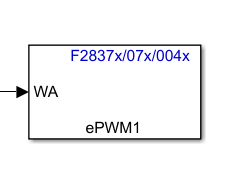
\includegraphics[width=1.8in]{sections/section6/images/SVPWM/ePWMBlock.png}
    \caption{ePWM block in Simulink}
    \label{fig:svpwm_block}
\end{figure}

\newpage